\documentclass{standalone}
\usepackage{tikz}
\usetikzlibrary{patterns, positioning}


\begin{document}
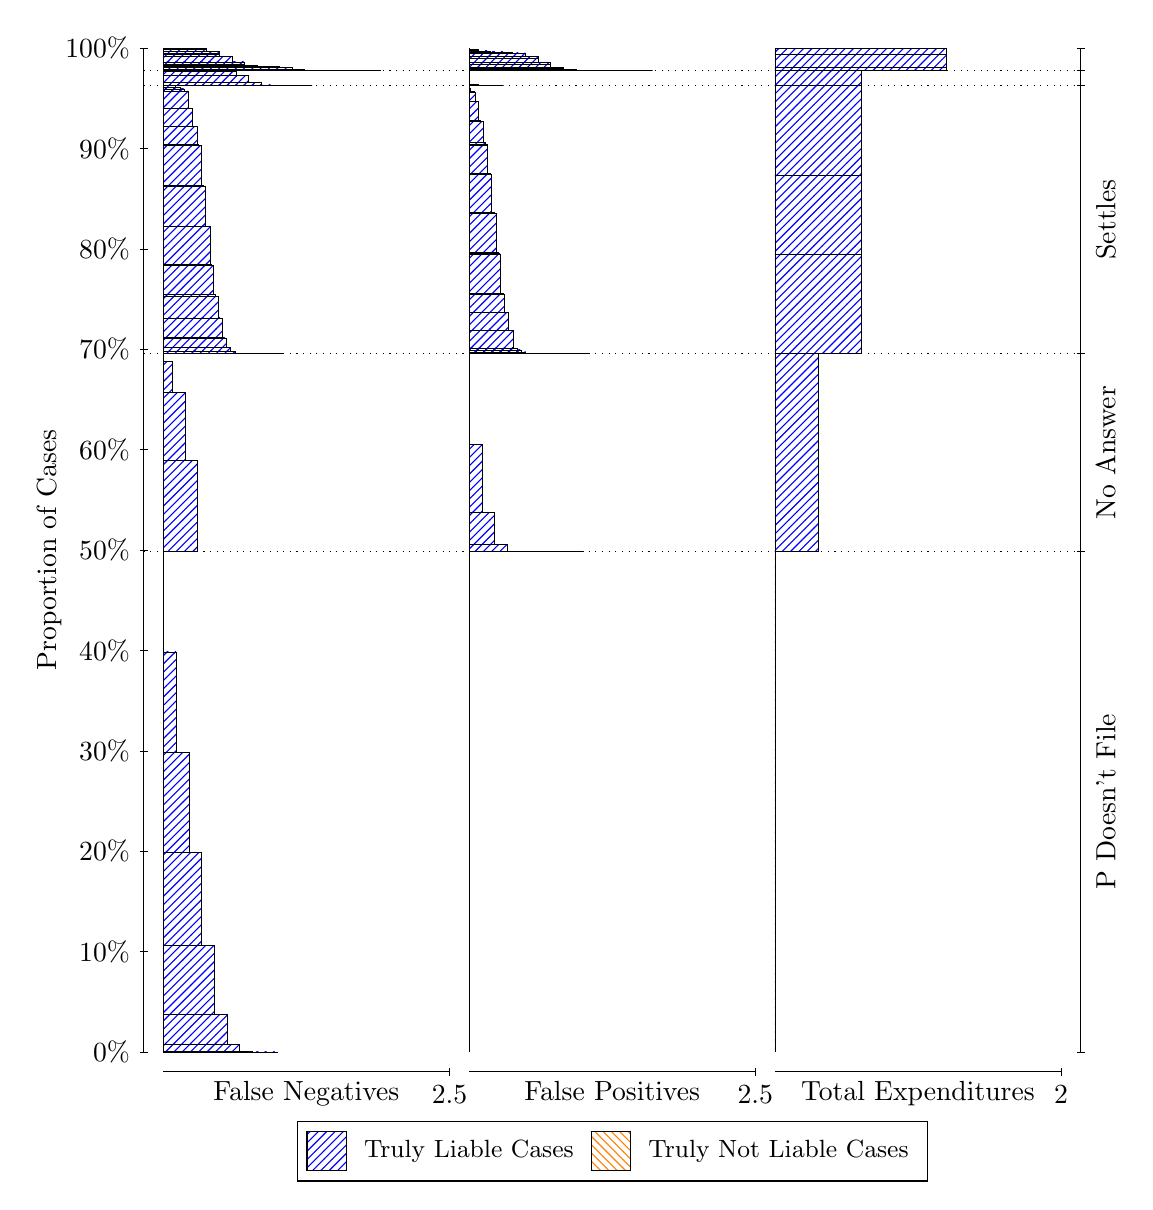
\begin{tikzpicture}
\draw[black, very thin] (1.5,1.75) -- (1.5,14.5);
\node[rotate=90, text=black, anchor=center] at (0.3, 8.125) {Proportion of Cases};
\draw[black, very thin] (1.45,1.75) -- (1.55,1.75);
\node[text=black, anchor=east] at (1.45, 1.75) {0\%};
\draw[black, very thin] (1.45,3.025) -- (1.55,3.025);
\node[text=black, anchor=east] at (1.45, 3.025) {10\%};
\draw[black, very thin] (1.45,4.3) -- (1.55,4.3);
\node[text=black, anchor=east] at (1.45, 4.3) {20\%};
\draw[black, very thin] (1.45,5.575) -- (1.55,5.575);
\node[text=black, anchor=east] at (1.45, 5.575) {30\%};
\draw[black, very thin] (1.45,6.85) -- (1.55,6.85);
\node[text=black, anchor=east] at (1.45, 6.85) {40\%};
\draw[black, very thin] (1.45,8.125) -- (1.55,8.125);
\node[text=black, anchor=east] at (1.45, 8.125) {50\%};
\draw[black, very thin] (1.45,9.4) -- (1.55,9.4);
\node[text=black, anchor=east] at (1.45, 9.4) {60\%};
\draw[black, very thin] (1.45,10.675) -- (1.55,10.675);
\node[text=black, anchor=east] at (1.45, 10.675) {70\%};
\draw[black, very thin] (1.45,11.95) -- (1.55,11.95);
\node[text=black, anchor=east] at (1.45, 11.95) {80\%};
\draw[black, very thin] (1.45,13.225) -- (1.55,13.225);
\node[text=black, anchor=east] at (1.45, 13.225) {90\%};
\draw[black, very thin] (1.45,14.5) -- (1.55,14.5);
\node[text=black, anchor=east] at (1.45, 14.5) {100\%};

\draw[black, very thin] (13.4,1.75) -- (13.4,14.5);
\draw[black, very thin] (13.35,1.75) -- (13.45,1.75);
\node[anchor=west] at (13.35, 1.75) {};
\draw[black, very thin] (13.35,8.1049) -- (13.45,8.1049);
\node[anchor=west] at (13.35, 8.1049) {};
\draw[black, very thin] (13.35,10.618) -- (13.45,10.618);
\node[anchor=west] at (13.35, 10.618) {};
\draw[black, very thin] (13.35,14.029) -- (13.45,14.029);
\node[anchor=west] at (13.35, 14.029) {};
\draw[black, very thin] (13.35,14.215) -- (13.45,14.215);
\node[anchor=west] at (13.35, 14.215) {};
\draw[black, very thin] (13.35,14.5) -- (13.45,14.5);
\node[anchor=west] at (13.35, 14.5) {};

\draw[black, very thin, pattern color=blue, pattern=north east lines] (1.75,1.75) rectangle (3.2033,1.75);
\draw[black, very thin, pattern color=blue, pattern=north east lines] (1.75,1.75) rectangle (3.0419,1.7503);
\draw[black, very thin, pattern color=blue, pattern=north east lines] (1.75,1.7503) rectangle (2.8804,1.7582);
\draw[black, very thin, pattern color=blue, pattern=north east lines] (1.75,1.7582) rectangle (2.7189,1.8421);
\draw[black, very thin, pattern color=blue, pattern=north east lines] (1.75,1.8421) rectangle (2.5574,2.2307);
\draw[black, very thin, pattern color=blue, pattern=north east lines] (1.75,2.2307) rectangle (2.3959,3.1046);
\draw[black, very thin, pattern color=blue, pattern=north east lines] (1.75,3.1046) rectangle (2.2344,4.2895);
\draw[black, very thin, pattern color=blue, pattern=north east lines] (1.75,4.2895) rectangle (2.073,5.5553);
\draw[black, very thin, pattern color=blue, pattern=north east lines] (1.75,5.5553) rectangle (1.9115,6.8299);
\draw[black, very thin, pattern color=orange, pattern=north west lines] (1.75,6.8299) rectangle (1.75,6.8299);
\draw[black, very thin, pattern color=blue, pattern=north east lines] (1.75,6.8299) rectangle (1.75,8.1049);
\draw[black, very thin, pattern color=blue, pattern=north east lines] (1.75,8.1049) rectangle (2.186,9.26);
\draw[black, very thin, pattern color=blue, pattern=north east lines] (1.75,9.26) rectangle (2.0245,10.123);
\draw[black, very thin, pattern color=blue, pattern=north east lines] (1.75,10.123) rectangle (1.863,10.523);
\draw[black, very thin, pattern color=orange, pattern=north west lines] (1.75,10.523) rectangle (1.75,10.523);
\draw[black, very thin, pattern color=blue, pattern=north east lines] (1.75,10.523) rectangle (1.75,10.618);
\draw[black, very thin, pattern color=blue, pattern=north east lines] (1.75,10.618) rectangle (3.276,10.618);
\draw[black, very thin, pattern color=blue, pattern=north east lines] (1.75,10.618) rectangle (3.2033,10.618);
\draw[black, very thin, pattern color=blue, pattern=north east lines] (1.75,10.618) rectangle (3.1307,10.618);
\draw[black, very thin, pattern color=blue, pattern=north east lines] (1.75,10.618) rectangle (3.1145,10.618);
\draw[black, very thin, pattern color=blue, pattern=north east lines] (1.75,10.618) rectangle (3.058,10.618);
\draw[black, very thin, pattern color=blue, pattern=north east lines] (1.75,10.618) rectangle (3.0419,10.618);
\draw[black, very thin, pattern color=blue, pattern=north east lines] (1.75,10.618) rectangle (2.9853,10.618);
\draw[black, very thin, pattern color=blue, pattern=north east lines] (1.75,10.618) rectangle (2.9692,10.618);
\draw[black, very thin, pattern color=blue, pattern=north east lines] (1.75,10.618) rectangle (2.953,10.618);
\draw[black, very thin, pattern color=blue, pattern=north east lines] (1.75,10.618) rectangle (2.9127,10.618);
\draw[black, very thin, pattern color=blue, pattern=north east lines] (1.75,10.618) rectangle (2.8965,10.618);
\draw[black, very thin, pattern color=blue, pattern=north east lines] (1.75,10.618) rectangle (2.8804,10.618);
\draw[black, very thin, pattern color=blue, pattern=north east lines] (1.75,10.618) rectangle (2.84,10.618);
\draw[black, very thin, pattern color=blue, pattern=north east lines] (1.75,10.618) rectangle (2.8239,10.619);
\draw[black, very thin, pattern color=blue, pattern=north east lines] (1.75,10.619) rectangle (2.8077,10.619);
\draw[black, very thin, pattern color=blue, pattern=north east lines] (1.75,10.619) rectangle (2.7916,10.619);
\draw[black, very thin, pattern color=blue, pattern=north east lines] (1.75,10.619) rectangle (2.7673,10.622);
\draw[black, very thin, pattern color=blue, pattern=north east lines] (1.75,10.622) rectangle (2.7512,10.622);
\draw[black, very thin, pattern color=blue, pattern=north east lines] (1.75,10.622) rectangle (2.735,10.622);
\draw[black, very thin, pattern color=blue, pattern=north east lines] (1.75,10.622) rectangle (2.7189,10.622);
\draw[black, very thin, pattern color=blue, pattern=north east lines] (1.75,10.622) rectangle (2.6785,10.622);
\draw[black, very thin, pattern color=blue, pattern=north east lines] (1.75,10.622) rectangle (2.6624,10.652);
\draw[black, very thin, pattern color=blue, pattern=north east lines] (1.75,10.652) rectangle (2.6462,10.652);
\draw[black, very thin, pattern color=blue, pattern=north east lines] (1.75,10.652) rectangle (2.6301,10.653);
\draw[black, very thin, pattern color=blue, pattern=north east lines] (1.75,10.653) rectangle (2.6059,10.694);
\draw[black, very thin, pattern color=blue, pattern=north east lines] (1.75,10.694) rectangle (2.5897,10.694);
\draw[black, very thin, pattern color=blue, pattern=north east lines] (1.75,10.694) rectangle (2.5736,10.703);
\draw[black, very thin, pattern color=blue, pattern=north east lines] (1.75,10.703) rectangle (2.5574,10.703);
\draw[black, very thin, pattern color=blue, pattern=north east lines] (1.75,10.703) rectangle (2.5493,10.82);
\draw[black, very thin, pattern color=blue, pattern=north east lines] (1.75,10.82) rectangle (2.517,10.824);
\draw[black, very thin, pattern color=blue, pattern=north east lines] (1.75,10.824) rectangle (2.5009,11.069);
\draw[black, very thin, pattern color=blue, pattern=north east lines] (1.75,11.069) rectangle (2.4847,11.073);
\draw[black, very thin, pattern color=blue, pattern=north east lines] (1.75,11.073) rectangle (2.4686,11.074);
\draw[black, very thin, pattern color=blue, pattern=north east lines] (1.75,11.074) rectangle (2.4444,11.348);
\draw[black, very thin, pattern color=blue, pattern=north east lines] (1.75,11.348) rectangle (2.4282,11.349);
\draw[black, very thin, pattern color=blue, pattern=north east lines] (1.75,11.349) rectangle (2.4121,11.375);
\draw[black, very thin, pattern color=blue, pattern=north east lines] (1.75,11.375) rectangle (2.3959,11.376);
\draw[black, very thin, pattern color=blue, pattern=north east lines] (1.75,11.376) rectangle (2.3879,11.737);
\draw[black, very thin, pattern color=blue, pattern=north east lines] (1.75,11.737) rectangle (2.3556,11.754);
\draw[black, very thin, pattern color=blue, pattern=north east lines] (1.75,11.754) rectangle (2.3394,12.231);
\draw[black, very thin, pattern color=blue, pattern=north east lines] (1.75,12.231) rectangle (2.3233,12.239);
\draw[black, very thin, pattern color=blue, pattern=north east lines] (1.75,12.239) rectangle (2.3071,12.241);
\draw[black, very thin, pattern color=blue, pattern=north east lines] (1.75,12.241) rectangle (2.2829,12.741);
\draw[black, very thin, pattern color=blue, pattern=north east lines] (1.75,12.741) rectangle (2.2667,12.742);
\draw[black, very thin, pattern color=blue, pattern=north east lines] (1.75,12.742) rectangle (2.2506,12.759);
\draw[black, very thin, pattern color=blue, pattern=north east lines] (1.75,12.759) rectangle (2.2344,12.76);
\draw[black, very thin, pattern color=blue, pattern=north east lines] (1.75,12.76) rectangle (2.2264,13.264);
\draw[black, very thin, pattern color=blue, pattern=north east lines] (1.75,13.264) rectangle (2.1941,13.276);
\draw[black, very thin, pattern color=blue, pattern=north east lines] (1.75,13.276) rectangle (2.1779,13.501);
\draw[black, very thin, pattern color=blue, pattern=north east lines] (1.75,13.501) rectangle (2.1618,13.504);
\draw[black, very thin, pattern color=blue, pattern=north east lines] (1.75,13.504) rectangle (2.1456,13.504);
\draw[black, very thin, pattern color=blue, pattern=north east lines] (1.75,13.504) rectangle (2.1214,13.734);
\draw[black, very thin, pattern color=blue, pattern=north east lines] (1.75,13.734) rectangle (2.1053,13.734);
\draw[black, very thin, pattern color=blue, pattern=north east lines] (1.75,13.734) rectangle (2.0891,13.736);
\draw[black, very thin, pattern color=blue, pattern=north east lines] (1.75,13.736) rectangle (2.073,13.737);
\draw[black, very thin, pattern color=blue, pattern=north east lines] (1.75,13.737) rectangle (2.0649,13.955);
\draw[black, very thin, pattern color=blue, pattern=north east lines] (1.75,13.955) rectangle (2.0326,13.957);
\draw[black, very thin, pattern color=blue, pattern=north east lines] (1.75,13.957) rectangle (2.0164,13.981);
\draw[black, very thin, pattern color=blue, pattern=north east lines] (1.75,13.981) rectangle (2.0003,13.981);
\draw[black, very thin, pattern color=blue, pattern=north east lines] (1.75,13.981) rectangle (1.9841,13.981);
\draw[black, very thin, pattern color=blue, pattern=north east lines] (1.75,13.981) rectangle (1.9599,14.005);
\draw[black, very thin, pattern color=blue, pattern=north east lines] (1.75,14.005) rectangle (1.9438,14.005);
\draw[black, very thin, pattern color=blue, pattern=north east lines] (1.75,14.005) rectangle (1.9276,14.005);
\draw[black, very thin, pattern color=blue, pattern=north east lines] (1.75,14.005) rectangle (1.9115,14.005);
\draw[black, very thin, pattern color=blue, pattern=north east lines] (1.75,14.005) rectangle (1.9034,14.027);
\draw[black, very thin, pattern color=blue, pattern=north east lines] (1.75,14.027) rectangle (1.8711,14.027);
\draw[black, very thin, pattern color=blue, pattern=north east lines] (1.75,14.027) rectangle (1.855,14.028);
\draw[black, very thin, pattern color=blue, pattern=north east lines] (1.75,14.028) rectangle (1.8388,14.028);
\draw[black, very thin, pattern color=blue, pattern=north east lines] (1.75,14.028) rectangle (1.8227,14.028);
\draw[black, very thin, pattern color=blue, pattern=north east lines] (1.75,14.028) rectangle (1.7984,14.028);
\draw[black, very thin, pattern color=blue, pattern=north east lines] (1.75,14.028) rectangle (1.7823,14.028);
\draw[black, very thin, pattern color=blue, pattern=north east lines] (1.75,14.028) rectangle (1.7661,14.028);
\draw[black, very thin, pattern color=orange, pattern=north west lines] (1.75,14.028) rectangle (1.75,14.028);
\draw[black, very thin, pattern color=blue, pattern=north east lines] (1.75,14.028) rectangle (1.75,14.029);
\draw[black, very thin, pattern color=blue, pattern=north east lines] (1.75,14.029) rectangle (3.6393,14.029);
\draw[black, very thin, pattern color=blue, pattern=north east lines] (1.75,14.029) rectangle (3.4779,14.029);
\draw[black, very thin, pattern color=blue, pattern=north east lines] (1.75,14.029) rectangle (3.3164,14.029);
\draw[black, very thin, pattern color=blue, pattern=north east lines] (1.75,14.029) rectangle (3.1549,14.031);
\draw[black, very thin, pattern color=blue, pattern=north east lines] (1.75,14.031) rectangle (2.9934,14.062);
\draw[black, very thin, pattern color=blue, pattern=north east lines] (1.75,14.062) rectangle (2.8319,14.154);
\draw[black, very thin, pattern color=blue, pattern=north east lines] (1.75,14.154) rectangle (2.6704,14.207);
\draw[black, very thin, pattern color=blue, pattern=north east lines] (1.75,14.207) rectangle (2.509,14.214);
\draw[black, very thin, pattern color=blue, pattern=north east lines] (1.75,14.214) rectangle (2.3475,14.215);
\draw[black, very thin, pattern color=blue, pattern=north east lines] (1.75,14.215) rectangle (2.186,14.215);
\draw[black, very thin, pattern color=orange, pattern=north west lines] (1.75,14.215) rectangle (1.75,14.215);
\draw[black, very thin, pattern color=blue, pattern=north east lines] (1.75,14.215) rectangle (4.5113,14.215);
\draw[black, very thin, pattern color=blue, pattern=north east lines] (1.75,14.215) rectangle (4.3499,14.215);
\draw[black, very thin, pattern color=blue, pattern=north east lines] (1.75,14.215) rectangle (4.1884,14.215);
\draw[black, very thin, pattern color=blue, pattern=north east lines] (1.75,14.215) rectangle (4.0269,14.215);
\draw[black, very thin, pattern color=blue, pattern=north east lines] (1.75,14.215) rectangle (4.0269,14.215);
\draw[black, very thin, pattern color=blue, pattern=north east lines] (1.75,14.215) rectangle (3.8654,14.215);
\draw[black, very thin, pattern color=blue, pattern=north east lines] (1.75,14.215) rectangle (3.8654,14.215);
\draw[black, very thin, pattern color=blue, pattern=north east lines] (1.75,14.215) rectangle (3.7524,14.215);
\draw[black, very thin, pattern color=blue, pattern=north east lines] (1.75,14.215) rectangle (3.7039,14.216);
\draw[black, very thin, pattern color=blue, pattern=north east lines] (1.75,14.216) rectangle (3.7039,14.217);
\draw[black, very thin, pattern color=blue, pattern=north east lines] (1.75,14.217) rectangle (3.5909,14.217);
\draw[black, very thin, pattern color=blue, pattern=north east lines] (1.75,14.217) rectangle (3.5424,14.227);
\draw[black, very thin, pattern color=blue, pattern=north east lines] (1.75,14.227) rectangle (3.5424,14.228);
\draw[black, very thin, pattern color=blue, pattern=north east lines] (1.75,14.228) rectangle (3.4294,14.228);
\draw[black, very thin, pattern color=blue, pattern=north east lines] (1.75,14.228) rectangle (3.381,14.25);
\draw[black, very thin, pattern color=blue, pattern=north east lines] (1.75,14.25) rectangle (3.381,14.25);
\draw[black, very thin, pattern color=blue, pattern=north east lines] (1.75,14.25) rectangle (3.2679,14.25);
\draw[black, very thin, pattern color=blue, pattern=north east lines] (1.75,14.25) rectangle (3.2679,14.25);
\draw[black, very thin, pattern color=blue, pattern=north east lines] (1.75,14.25) rectangle (3.2195,14.265);
\draw[black, very thin, pattern color=blue, pattern=north east lines] (1.75,14.265) rectangle (3.1064,14.265);
\draw[black, very thin, pattern color=blue, pattern=north east lines] (1.75,14.265) rectangle (3.1064,14.265);
\draw[black, very thin, pattern color=blue, pattern=north east lines] (1.75,14.265) rectangle (3.058,14.267);
\draw[black, very thin, pattern color=blue, pattern=north east lines] (1.75,14.267) rectangle (2.945,14.277);
\draw[black, very thin, pattern color=blue, pattern=north east lines] (1.75,14.277) rectangle (2.8965,14.277);
\draw[black, very thin, pattern color=blue, pattern=north east lines] (1.75,14.277) rectangle (2.8965,14.277);
\draw[black, very thin, pattern color=blue, pattern=north east lines] (1.75,14.277) rectangle (2.7835,14.295);
\draw[black, very thin, pattern color=blue, pattern=north east lines] (1.75,14.295) rectangle (2.7835,14.324);
\draw[black, very thin, pattern color=blue, pattern=north east lines] (1.75,14.324) rectangle (2.735,14.324);
\draw[black, very thin, pattern color=blue, pattern=north east lines] (1.75,14.324) rectangle (2.735,14.324);
\draw[black, very thin, pattern color=blue, pattern=north east lines] (1.75,14.324) rectangle (2.622,14.398);
\draw[black, very thin, pattern color=blue, pattern=north east lines] (1.75,14.398) rectangle (2.5736,14.398);
\draw[black, very thin, pattern color=blue, pattern=north east lines] (1.75,14.398) rectangle (2.4605,14.426);
\draw[black, very thin, pattern color=blue, pattern=north east lines] (1.75,14.426) rectangle (2.4605,14.427);
\draw[black, very thin, pattern color=blue, pattern=north east lines] (1.75,14.427) rectangle (2.4605,14.459);
\draw[black, very thin, pattern color=blue, pattern=north east lines] (1.75,14.459) rectangle (2.4121,14.459);
\draw[black, very thin, pattern color=blue, pattern=north east lines] (1.75,14.459) rectangle (2.299,14.49);
\draw[black, very thin, pattern color=blue, pattern=north east lines] (1.75,14.49) rectangle (2.299,14.491);
\draw[black, very thin, pattern color=blue, pattern=north east lines] (1.75,14.491) rectangle (2.1376,14.493);
\draw[black, very thin, pattern color=blue, pattern=north east lines] (1.75,14.493) rectangle (2.1376,14.494);
\draw[black, very thin, pattern color=blue, pattern=north east lines] (1.75,14.494) rectangle (2.1376,14.499);
\draw[black, very thin, pattern color=blue, pattern=north east lines] (1.75,14.499) rectangle (1.9761,14.5);
\draw[black, very thin, pattern color=blue, pattern=north east lines] (1.75,14.5) rectangle (1.9761,14.5);
\draw[black, very thin, pattern color=blue, pattern=north east lines] (1.75,14.5) rectangle (1.8146,14.5);
\draw[black, very thin, pattern color=blue, pattern=north east lines] (1.75,14.5) rectangle (1.8146,14.5);
\draw[black, very thin, pattern color=orange, pattern=north west lines] (1.75,14.5) rectangle (1.75,14.5);
\draw[black, very thin, pattern color=blue, pattern=north east lines] (1.75,14.5) rectangle (1.75,14.5);
\draw[black, very thin, pattern color=orange, pattern=north west lines] (5.6333,1.75) rectangle (5.6333,1.75);
\draw[black, very thin, pattern color=blue, pattern=north east lines] (5.6333,1.75) rectangle (5.6333,8.1049);
\draw[black, very thin, pattern color=orange, pattern=north west lines] (5.6333,8.1049) rectangle (7.0867,8.1049);
\draw[black, very thin, pattern color=blue, pattern=north east lines] (5.6333,8.1049) rectangle (7.0867,8.1049);
\draw[black, very thin, pattern color=blue, pattern=north east lines] (5.6333,8.1049) rectangle (6.9252,8.1049);
\draw[black, very thin, pattern color=blue, pattern=north east lines] (5.6333,8.1049) rectangle (6.7637,8.1049);
\draw[black, very thin, pattern color=blue, pattern=north east lines] (5.6333,8.1049) rectangle (6.6022,8.1049);
\draw[black, very thin, pattern color=blue, pattern=north east lines] (5.6333,8.1049) rectangle (6.4407,8.105);
\draw[black, very thin, pattern color=blue, pattern=north east lines] (5.6333,8.105) rectangle (6.2793,8.1121);
\draw[black, very thin, pattern color=blue, pattern=north east lines] (5.6333,8.1121) rectangle (6.1178,8.2);
\draw[black, very thin, pattern color=blue, pattern=north east lines] (5.6333,8.2) rectangle (5.9563,8.6);
\draw[black, very thin, pattern color=blue, pattern=north east lines] (5.6333,8.6) rectangle (5.7948,9.4631);
\draw[black, very thin, pattern color=blue, pattern=north east lines] (5.6333,9.4631) rectangle (5.6333,10.618);
\draw[black, very thin, pattern color=orange, pattern=north west lines] (5.6333,10.618) rectangle (7.1593,10.618);
\draw[black, very thin, pattern color=blue, pattern=north east lines] (5.6333,10.618) rectangle (7.1593,10.618);
\draw[black, very thin, pattern color=blue, pattern=north east lines] (5.6333,10.618) rectangle (6.9979,10.618);
\draw[black, very thin, pattern color=orange, pattern=north west lines] (5.6333,10.618) rectangle (6.9413,10.618);
\draw[black, very thin, pattern color=blue, pattern=north east lines] (5.6333,10.618) rectangle (6.9413,10.618);
\draw[black, very thin, pattern color=orange, pattern=north west lines] (5.6333,10.618) rectangle (6.8687,10.618);
\draw[black, very thin, pattern color=blue, pattern=north east lines] (5.6333,10.618) rectangle (6.8687,10.618);
\draw[black, very thin, pattern color=blue, pattern=north east lines] (5.6333,10.618) rectangle (6.8364,10.618);
\draw[black, very thin, pattern color=orange, pattern=north west lines] (5.6333,10.618) rectangle (6.796,10.618);
\draw[black, very thin, pattern color=blue, pattern=north east lines] (5.6333,10.618) rectangle (6.796,10.618);
\draw[black, very thin, pattern color=blue, pattern=north east lines] (5.6333,10.618) rectangle (6.7799,10.618);
\draw[black, very thin, pattern color=orange, pattern=north west lines] (5.6333,10.618) rectangle (6.7233,10.618);
\draw[black, very thin, pattern color=blue, pattern=north east lines] (5.6333,10.618) rectangle (6.7233,10.618);
\draw[black, very thin, pattern color=blue, pattern=north east lines] (5.6333,10.618) rectangle (6.7072,10.618);
\draw[black, very thin, pattern color=blue, pattern=north east lines] (5.6333,10.618) rectangle (6.6749,10.618);
\draw[black, very thin, pattern color=orange, pattern=north west lines] (5.6333,10.618) rectangle (6.6507,10.618);
\draw[black, very thin, pattern color=blue, pattern=north east lines] (5.6333,10.618) rectangle (6.6507,10.618);
\draw[black, very thin, pattern color=blue, pattern=north east lines] (5.6333,10.618) rectangle (6.6345,10.618);
\draw[black, very thin, pattern color=blue, pattern=north east lines] (5.6333,10.618) rectangle (6.6184,10.618);
\draw[black, very thin, pattern color=orange, pattern=north west lines] (5.6333,10.618) rectangle (6.578,10.618);
\draw[black, very thin, pattern color=blue, pattern=north east lines] (5.6333,10.618) rectangle (6.578,10.618);
\draw[black, very thin, pattern color=blue, pattern=north east lines] (5.6333,10.618) rectangle (6.5619,10.618);
\draw[black, very thin, pattern color=blue, pattern=north east lines] (5.6333,10.618) rectangle (6.5457,10.618);
\draw[black, very thin, pattern color=blue, pattern=north east lines] (5.6333,10.618) rectangle (6.5134,10.619);
\draw[black, very thin, pattern color=orange, pattern=north west lines] (5.6333,10.619) rectangle (6.5053,10.619);
\draw[black, very thin, pattern color=blue, pattern=north east lines] (5.6333,10.619) rectangle (6.5053,10.619);
\draw[black, very thin, pattern color=blue, pattern=north east lines] (5.6333,10.619) rectangle (6.4892,10.619);
\draw[black, very thin, pattern color=blue, pattern=north east lines] (5.6333,10.619) rectangle (6.473,10.619);
\draw[black, very thin, pattern color=blue, pattern=north east lines] (5.6333,10.619) rectangle (6.4569,10.619);
\draw[black, very thin, pattern color=orange, pattern=north west lines] (5.6333,10.619) rectangle (6.4327,10.619);
\draw[black, very thin, pattern color=blue, pattern=north east lines] (5.6333,10.619) rectangle (6.4327,10.619);
\draw[black, very thin, pattern color=blue, pattern=north east lines] (5.6333,10.619) rectangle (6.4165,10.619);
\draw[black, very thin, pattern color=blue, pattern=north east lines] (5.6333,10.619) rectangle (6.4004,10.62);
\draw[black, very thin, pattern color=blue, pattern=north east lines] (5.6333,10.62) rectangle (6.3842,10.62);
\draw[black, very thin, pattern color=blue, pattern=north east lines] (5.6333,10.62) rectangle (6.3519,10.642);
\draw[black, very thin, pattern color=blue, pattern=north east lines] (5.6333,10.642) rectangle (6.3439,10.642);
\draw[black, very thin, pattern color=blue, pattern=north east lines] (5.6333,10.642) rectangle (6.3277,10.642);
\draw[black, very thin, pattern color=blue, pattern=north east lines] (5.6333,10.642) rectangle (6.3116,10.642);
\draw[black, very thin, pattern color=blue, pattern=north east lines] (5.6333,10.642) rectangle (6.2954,10.666);
\draw[black, very thin, pattern color=blue, pattern=north east lines] (5.6333,10.666) rectangle (6.2712,10.666);
\draw[black, very thin, pattern color=blue, pattern=north east lines] (5.6333,10.666) rectangle (6.255,10.667);
\draw[black, very thin, pattern color=blue, pattern=north east lines] (5.6333,10.667) rectangle (6.2389,10.69);
\draw[black, very thin, pattern color=blue, pattern=north east lines] (5.6333,10.69) rectangle (6.2227,10.692);
\draw[black, very thin, pattern color=blue, pattern=north east lines] (5.6333,10.692) rectangle (6.1904,10.911);
\draw[black, very thin, pattern color=blue, pattern=north east lines] (5.6333,10.911) rectangle (6.1824,10.911);
\draw[black, very thin, pattern color=blue, pattern=north east lines] (5.6333,10.911) rectangle (6.1662,10.913);
\draw[black, very thin, pattern color=blue, pattern=north east lines] (5.6333,10.913) rectangle (6.1501,10.913);
\draw[black, very thin, pattern color=blue, pattern=north east lines] (5.6333,10.913) rectangle (6.1339,11.143);
\draw[black, very thin, pattern color=blue, pattern=north east lines] (5.6333,11.143) rectangle (6.1097,11.143);
\draw[black, very thin, pattern color=blue, pattern=north east lines] (5.6333,11.143) rectangle (6.0936,11.146);
\draw[black, very thin, pattern color=blue, pattern=north east lines] (5.6333,11.146) rectangle (6.0774,11.371);
\draw[black, very thin, pattern color=blue, pattern=north east lines] (5.6333,11.371) rectangle (6.0613,11.384);
\draw[black, very thin, pattern color=blue, pattern=north east lines] (5.6333,11.384) rectangle (6.029,11.887);
\draw[black, very thin, pattern color=blue, pattern=north east lines] (5.6333,11.887) rectangle (6.0209,11.889);
\draw[black, very thin, pattern color=blue, pattern=north east lines] (5.6333,11.889) rectangle (6.0047,11.905);
\draw[black, very thin, pattern color=blue, pattern=north east lines] (5.6333,11.905) rectangle (5.9886,11.907);
\draw[black, very thin, pattern color=blue, pattern=north east lines] (5.6333,11.907) rectangle (5.9724,12.406);
\draw[black, very thin, pattern color=blue, pattern=north east lines] (5.6333,12.406) rectangle (5.9482,12.408);
\draw[black, very thin, pattern color=blue, pattern=north east lines] (5.6333,12.408) rectangle (5.9321,12.416);
\draw[black, very thin, pattern color=blue, pattern=north east lines] (5.6333,12.416) rectangle (5.9159,12.893);
\draw[black, very thin, pattern color=blue, pattern=north east lines] (5.6333,12.893) rectangle (5.8998,12.91);
\draw[black, very thin, pattern color=blue, pattern=north east lines] (5.6333,12.91) rectangle (5.8675,13.271);
\draw[black, very thin, pattern color=blue, pattern=north east lines] (5.6333,13.271) rectangle (5.8594,13.272);
\draw[black, very thin, pattern color=blue, pattern=north east lines] (5.6333,13.272) rectangle (5.8433,13.298);
\draw[black, very thin, pattern color=blue, pattern=north east lines] (5.6333,13.298) rectangle (5.8271,13.299);
\draw[black, very thin, pattern color=blue, pattern=north east lines] (5.6333,13.299) rectangle (5.811,13.573);
\draw[black, very thin, pattern color=blue, pattern=north east lines] (5.6333,13.573) rectangle (5.7867,13.574);
\draw[black, very thin, pattern color=blue, pattern=north east lines] (5.6333,13.574) rectangle (5.7706,13.579);
\draw[black, very thin, pattern color=blue, pattern=north east lines] (5.6333,13.579) rectangle (5.7544,13.823);
\draw[black, very thin, pattern color=blue, pattern=north east lines] (5.6333,13.823) rectangle (5.7383,13.827);
\draw[black, very thin, pattern color=blue, pattern=north east lines] (5.6333,13.827) rectangle (5.706,13.944);
\draw[black, very thin, pattern color=blue, pattern=north east lines] (5.6333,13.944) rectangle (5.6979,13.945);
\draw[black, very thin, pattern color=blue, pattern=north east lines] (5.6333,13.945) rectangle (5.6818,13.953);
\draw[black, very thin, pattern color=blue, pattern=north east lines] (5.6333,13.953) rectangle (5.6656,13.953);
\draw[black, very thin, pattern color=blue, pattern=north east lines] (5.6333,13.953) rectangle (5.6495,13.995);
\draw[black, very thin, pattern color=blue, pattern=north east lines] (5.6333,13.995) rectangle (5.6333,14.029);
\draw[black, very thin, pattern color=orange, pattern=north west lines] (5.6333,14.029) rectangle (6.0693,14.029);
\draw[black, very thin, pattern color=blue, pattern=north east lines] (5.6333,14.029) rectangle (6.0693,14.029);
\draw[black, very thin, pattern color=blue, pattern=north east lines] (5.6333,14.029) rectangle (5.9079,14.029);
\draw[black, very thin, pattern color=blue, pattern=north east lines] (5.6333,14.029) rectangle (5.7464,14.037);
\draw[black, very thin, pattern color=blue, pattern=north east lines] (5.6333,14.037) rectangle (5.6333,14.215);
\draw[black, very thin, pattern color=orange, pattern=north west lines] (5.6333,14.215) rectangle (7.9587,14.215);
\draw[black, very thin, pattern color=blue, pattern=north east lines] (5.6333,14.215) rectangle (7.9587,14.215);
\draw[black, very thin, pattern color=orange, pattern=north west lines] (5.6333,14.215) rectangle (7.7972,14.215);
\draw[black, very thin, pattern color=blue, pattern=north east lines] (5.6333,14.215) rectangle (7.7972,14.215);
\draw[black, very thin, pattern color=orange, pattern=north west lines] (5.6333,14.215) rectangle (7.6357,14.215);
\draw[black, very thin, pattern color=blue, pattern=north east lines] (5.6333,14.215) rectangle (7.6357,14.215);
\draw[black, very thin, pattern color=blue, pattern=north east lines] (5.6333,14.215) rectangle (7.4742,14.215);
\draw[black, very thin, pattern color=orange, pattern=north west lines] (5.6333,14.215) rectangle (7.4742,14.215);
\draw[black, very thin, pattern color=blue, pattern=north east lines] (5.6333,14.215) rectangle (7.4742,14.215);
\draw[black, very thin, pattern color=blue, pattern=north east lines] (5.6333,14.215) rectangle (7.3127,14.215);
\draw[black, very thin, pattern color=orange, pattern=north west lines] (5.6333,14.215) rectangle (7.3127,14.215);
\draw[black, very thin, pattern color=blue, pattern=north east lines] (5.6333,14.215) rectangle (7.3127,14.215);
\draw[black, very thin, pattern color=blue, pattern=north east lines] (5.6333,14.215) rectangle (7.1513,14.216);
\draw[black, very thin, pattern color=orange, pattern=north west lines] (5.6333,14.216) rectangle (7.1513,14.216);
\draw[black, very thin, pattern color=blue, pattern=north east lines] (5.6333,14.216) rectangle (7.1513,14.216);
\draw[black, very thin, pattern color=blue, pattern=north east lines] (5.6333,14.216) rectangle (6.9898,14.22);
\draw[black, very thin, pattern color=orange, pattern=north west lines] (5.6333,14.22) rectangle (6.9898,14.22);
\draw[black, very thin, pattern color=blue, pattern=north east lines] (5.6333,14.22) rectangle (6.9898,14.224);
\draw[black, very thin, pattern color=blue, pattern=north east lines] (5.6333,14.224) rectangle (6.9898,14.224);
\draw[black, very thin, pattern color=blue, pattern=north east lines] (5.6333,14.224) rectangle (6.9898,14.224);
\draw[black, very thin, pattern color=blue, pattern=north east lines] (5.6333,14.224) rectangle (6.8283,14.243);
\draw[black, very thin, pattern color=orange, pattern=north west lines] (5.6333,14.243) rectangle (6.8283,14.243);
\draw[black, very thin, pattern color=blue, pattern=north east lines] (5.6333,14.243) rectangle (6.8283,14.255);
\draw[black, very thin, pattern color=blue, pattern=north east lines] (5.6333,14.255) rectangle (6.8283,14.255);
\draw[black, very thin, pattern color=orange, pattern=north west lines] (5.6333,14.255) rectangle (6.7153,14.255);
\draw[black, very thin, pattern color=blue, pattern=north east lines] (5.6333,14.255) rectangle (6.7153,14.255);
\draw[black, very thin, pattern color=blue, pattern=north east lines] (5.6333,14.255) rectangle (6.6668,14.257);
\draw[black, very thin, pattern color=blue, pattern=north east lines] (5.6333,14.257) rectangle (6.6668,14.293);
\draw[black, very thin, pattern color=blue, pattern=north east lines] (5.6333,14.293) rectangle (6.6668,14.317);
\draw[black, very thin, pattern color=orange, pattern=north west lines] (5.6333,14.317) rectangle (6.5538,14.317);
\draw[black, very thin, pattern color=blue, pattern=north east lines] (5.6333,14.317) rectangle (6.5538,14.317);
\draw[black, very thin, pattern color=blue, pattern=north east lines] (5.6333,14.317) rectangle (6.5053,14.32);
\draw[black, very thin, pattern color=blue, pattern=north east lines] (5.6333,14.32) rectangle (6.5053,14.365);
\draw[black, very thin, pattern color=blue, pattern=north east lines] (5.6333,14.365) rectangle (6.5053,14.391);
\draw[black, very thin, pattern color=blue, pattern=north east lines] (5.6333,14.391) rectangle (6.3923,14.391);
\draw[black, very thin, pattern color=orange, pattern=north west lines] (5.6333,14.391) rectangle (6.3923,14.391);
\draw[black, very thin, pattern color=blue, pattern=north east lines] (5.6333,14.391) rectangle (6.3923,14.391);
\draw[black, very thin, pattern color=blue, pattern=north east lines] (5.6333,14.391) rectangle (6.3439,14.396);
\draw[black, very thin, pattern color=blue, pattern=north east lines] (5.6333,14.396) rectangle (6.3439,14.396);
\draw[black, very thin, pattern color=blue, pattern=north east lines] (5.6333,14.396) rectangle (6.3439,14.432);
\draw[black, very thin, pattern color=blue, pattern=north east lines] (5.6333,14.432) rectangle (6.3439,14.438);
\draw[black, very thin, pattern color=blue, pattern=north east lines] (5.6333,14.438) rectangle (6.2308,14.438);
\draw[black, very thin, pattern color=orange, pattern=north west lines] (5.6333,14.438) rectangle (6.2308,14.438);
\draw[black, very thin, pattern color=blue, pattern=north east lines] (5.6333,14.438) rectangle (6.2308,14.438);
\draw[black, very thin, pattern color=blue, pattern=north east lines] (5.6333,14.438) rectangle (6.2308,14.438);
\draw[black, very thin, pattern color=blue, pattern=north east lines] (5.6333,14.438) rectangle (6.1824,14.441);
\draw[black, very thin, pattern color=blue, pattern=north east lines] (5.6333,14.441) rectangle (6.1824,14.448);
\draw[black, very thin, pattern color=blue, pattern=north east lines] (5.6333,14.448) rectangle (6.0693,14.449);
\draw[black, very thin, pattern color=orange, pattern=north west lines] (5.6333,14.449) rectangle (6.0693,14.449);
\draw[black, very thin, pattern color=blue, pattern=north east lines] (5.6333,14.449) rectangle (6.0693,14.45);
\draw[black, very thin, pattern color=blue, pattern=north east lines] (5.6333,14.45) rectangle (6.0693,14.45);
\draw[black, very thin, pattern color=blue, pattern=north east lines] (5.6333,14.45) rectangle (6.0209,14.45);
\draw[black, very thin, pattern color=blue, pattern=north east lines] (5.6333,14.45) rectangle (6.0209,14.45);
\draw[black, very thin, pattern color=blue, pattern=north east lines] (5.6333,14.45) rectangle (6.0209,14.45);
\draw[black, very thin, pattern color=blue, pattern=north east lines] (5.6333,14.45) rectangle (5.9079,14.464);
\draw[black, very thin, pattern color=blue, pattern=north east lines] (5.6333,14.464) rectangle (5.9079,14.464);
\draw[black, very thin, pattern color=blue, pattern=north east lines] (5.6333,14.464) rectangle (5.8594,14.464);
\draw[black, very thin, pattern color=blue, pattern=north east lines] (5.6333,14.464) rectangle (5.8594,14.464);
\draw[black, very thin, pattern color=blue, pattern=north east lines] (5.6333,14.464) rectangle (5.7464,14.476);
\draw[black, very thin, pattern color=blue, pattern=north east lines] (5.6333,14.476) rectangle (5.7464,14.477);
\draw[black, very thin, pattern color=blue, pattern=north east lines] (5.6333,14.477) rectangle (5.7464,14.487);
\draw[black, very thin, pattern color=blue, pattern=north east lines] (5.6333,14.487) rectangle (5.6979,14.487);
\draw[black, very thin, pattern color=blue, pattern=north east lines] (5.6333,14.487) rectangle (5.6979,14.487);
\draw[black, very thin, pattern color=blue, pattern=north east lines] (5.6333,14.487) rectangle (5.6979,14.487);
\draw[black, very thin, pattern color=blue, pattern=north east lines] (5.6333,14.487) rectangle (5.6333,14.5);
\draw[black, very thin, pattern color=orange, pattern=north west lines] (9.5167,1.75) rectangle (9.5167,1.75);
\draw[black, very thin, pattern color=blue, pattern=north east lines] (9.5167,1.75) rectangle (9.5167,8.1049);
\draw[black, very thin, pattern color=orange, pattern=north west lines] (9.5167,8.1049) rectangle (10.062,8.1049);
\draw[black, very thin, pattern color=blue, pattern=north east lines] (9.5167,8.1049) rectangle (10.062,10.618);
\draw[black, very thin, pattern color=orange, pattern=north west lines] (9.5167,10.618) rectangle (10.607,10.618);
\draw[black, very thin, pattern color=blue, pattern=north east lines] (9.5167,10.618) rectangle (10.607,11.883);
\draw[black, very thin, pattern color=orange, pattern=north west lines] (9.5167,11.883) rectangle (10.607,11.883);
\draw[black, very thin, pattern color=blue, pattern=north east lines] (9.5167,11.883) rectangle (10.607,12.887);
\draw[black, very thin, pattern color=orange, pattern=north west lines] (9.5167,12.887) rectangle (10.607,12.887);
\draw[black, very thin, pattern color=blue, pattern=north east lines] (9.5167,12.887) rectangle (10.607,14.029);
\draw[black, very thin, pattern color=orange, pattern=north west lines] (9.5167,14.029) rectangle (10.607,14.029);
\draw[black, very thin, pattern color=blue, pattern=north east lines] (9.5167,14.029) rectangle (10.607,14.215);
\draw[black, very thin, pattern color=orange, pattern=north west lines] (9.5167,14.215) rectangle (11.697,14.215);
\draw[black, very thin, pattern color=blue, pattern=north east lines] (9.5167,14.215) rectangle (11.697,14.259);
\draw[black, very thin, pattern color=orange, pattern=north west lines] (9.5167,14.259) rectangle (11.697,14.259);
\draw[black, very thin, pattern color=blue, pattern=north east lines] (9.5167,14.259) rectangle (11.697,14.419);
\draw[black, very thin, pattern color=orange, pattern=north west lines] (9.5167,14.419) rectangle (11.697,14.419);
\draw[black, very thin, pattern color=blue, pattern=north east lines] (9.5167,14.419) rectangle (11.697,14.5);
\draw[black, dotted] (1.5,8.1049) -- (13.4,8.1049);
\draw[black, dotted] (1.5,10.618) -- (13.4,10.618);
\draw[black, dotted] (1.5,14.029) -- (13.4,14.029);
\draw[black, dotted] (1.5,14.215) -- (13.4,14.215);
\draw[black, very thin] (1.75,1.5) -- (5.3833,1.5);
\node[text=black, anchor=north] at (3.5667, 1.5) {False Negatives};
\draw[black, very thin] (5.3833,1.45) -- (5.3833,1.55);
\node[text=black, anchor=north] at (5.3833, 1.45) {2.5};

\draw[black, very thin] (5.6333,1.5) -- (9.2667,1.5);
\node[text=black, anchor=north] at (7.45, 1.5) {False Positives};
\draw[black, very thin] (9.2667,1.45) -- (9.2667,1.55);
\node[text=black, anchor=north] at (9.2667, 1.45) {2.5};

\draw[black, very thin] (9.5167,1.5) -- (13.15,1.5);
\node[text=black, anchor=north] at (11.333, 1.5) {Total Expenditures};
\draw[black, very thin] (13.15,1.45) -- (13.15,1.55);
\node[text=black, anchor=north] at (13.15, 1.45) {2};

\node[text=black, centered, rotate=90] at (13.72, 4.9274) {P Doesn't File};
\node[text=black, centered, rotate=90] at (13.72, 9.3615) {No Answer};
\node[text=black, centered, rotate=90] at (13.72, 12.324) {Settles};



\draw (7.449999999999999,1.5) node[draw=none] (baseCoordinate) {};
\begin{scope}[align=center]
        \matrix[scale=0.5, draw=black, below=0.5cm of baseCoordinate, nodes={draw}, column sep=0.1cm]{
            \node[rectangle, draw, minimum width=0.5cm, minimum height=0.5cm, pattern color=blue, pattern=north east lines] {}; &
            \node[draw=none, font=\small, text=black] (B) {Truly Liable Cases}; &
            \node[rectangle, draw, minimum width=0.5cm, minimum height=0.5cm, pattern color=orange, pattern=north west lines] {}; &
            \node[draw=none, font=\small, text=black] (B) {Truly Not Liable Cases}; \\
            };
\end{scope}

\end{tikzpicture}
\end{document}